\documentclass{article}

\usepackage{multicol}
\usepackage{lipsum}
\usepackage{graphicx}
\graphicspath{{images/}}
\usepackage{blindtext}
\usepackage{subfiles} % Best loaded last in the preamble
\usepackage[dvipsnames]{xcolor}
\usepackage[T1]{fontenc}
\usepackage{setspace}
\usepackage{float}

\setlength{\columnsep}{1cm}

\usepackage{fullpage, tikz}
\usepackage{eso-pic}
\AddToShipoutPictureBG{%
	\begin{tikzpicture}[remember picture, overlay]
		\node[opacity=.4, inner sep=0pt]
		at(current page.center){
\includegraphics[width=8.5in, height=11in]{images/background}};
	\end{tikzpicture}%
}

\usepackage[margin={1.5cm,1.5cm}]{geometry}

\newcommand\BackgroundPic{%
	\put(0,0){%
		\parbox[b][\paperheight]{\paperwidth}{%
			\vfill
			\centering
			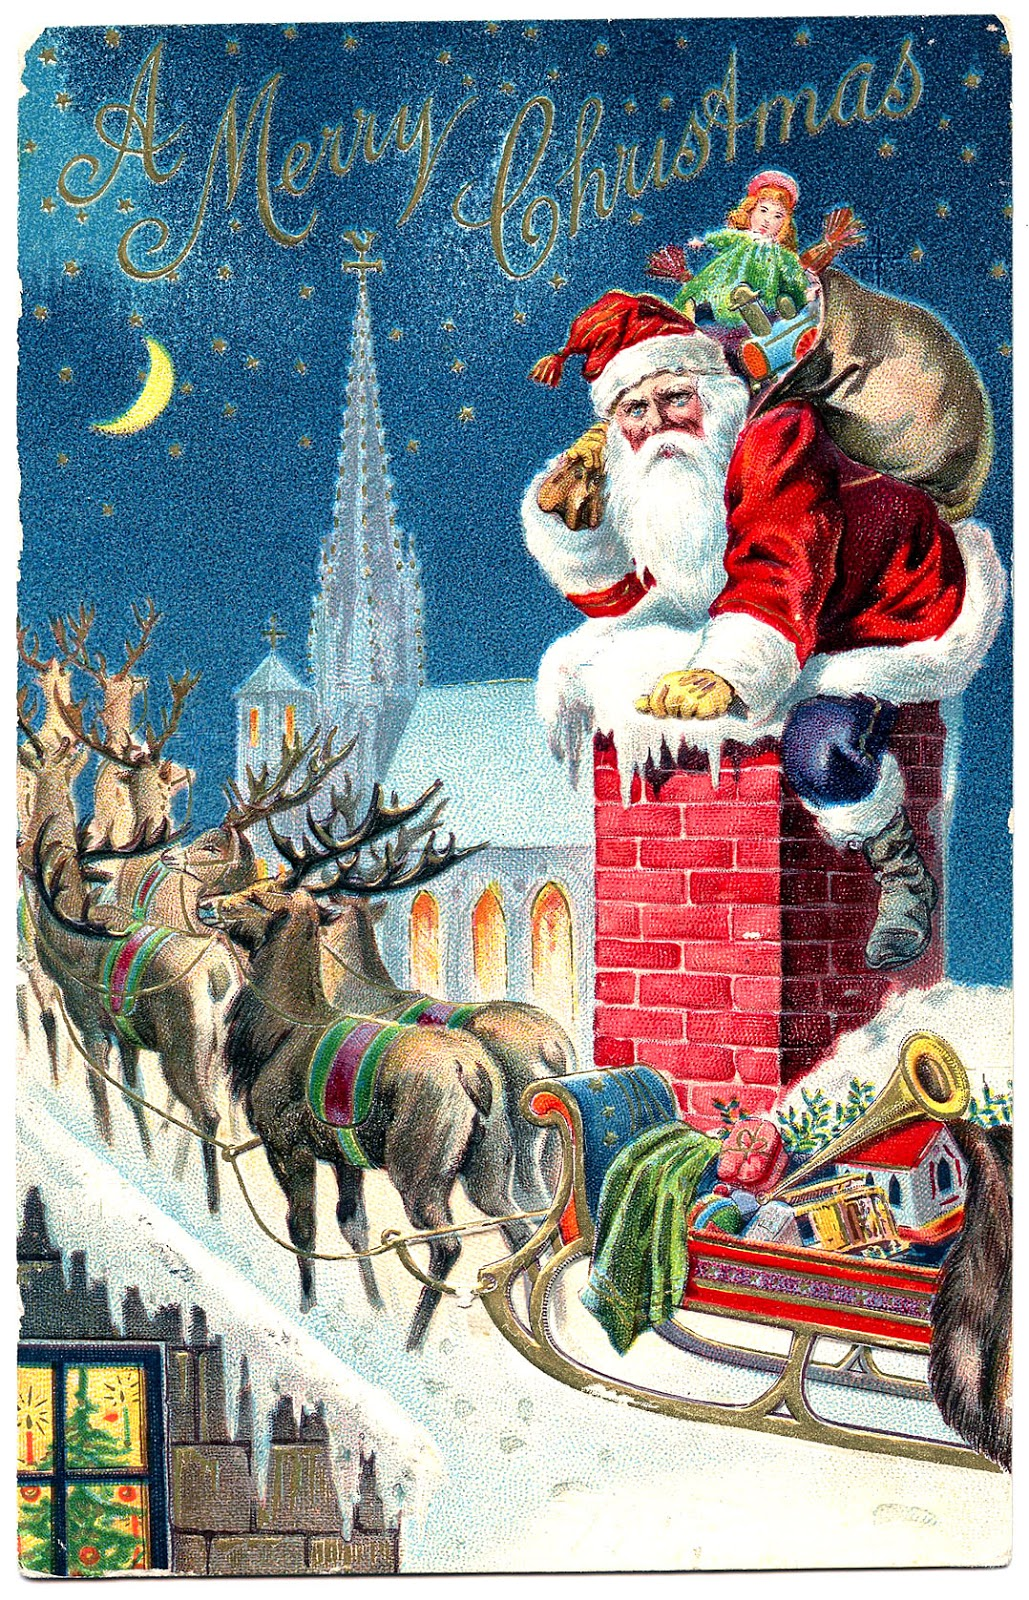
\includegraphics[width=\paperwidth,height=\paperheight]{images/cover.jpg}%
			\vfill
}}}

\title{\color{white}\textsc{\Huge Winter Solstice Sabotage }}
\date{ }


\setlength\fboxsep{8pt}

\begin{document}
	\AddToShipoutPicture*{\BackgroundPic}
	\maketitle
	\pagebreak
	\begin{multicols*}{2}
	\section{Introduction}
	
	\subsection*{Overview}
	The \emph{Winter Solstice Sabotage} one-off adventures is meant to be played with a group of 5 players at level 4. The adventure is meant to be completed in one session.
	
	It is a Christmas inspired story with familiar themes and characters. The plot of the story revolves around the character \emph{Klauss Atnas} (Santa Claus) whom has lost his powers to an evil gnome named \emph{Mister Frink}. The adventurers must help \emph{Klauss} find the evil gnome and defeat him to lift the curse and restore the blessing of the winter solstice.
	
	\subsection*{Adventure Hook}
	After a long year of adventures and treasure hunting, the adventurers find themselves returning home to celebrate the winter solstice when they are caught in a massive blizzard. They are forced to stop and find shelter, and happen to come across a tavern called the \emph{The Jolly Reindeer}. They enjoy a quiet meal with other guests lost in the storm when suddenly they hear a loud thump on which appears to come from the roof. Terrified, the hosts and other patrons try to convince the adventurers to go investigate what caused the loud noise on the roof.
	
	Upon investigating they find Klauss Atnas (Santa Claus) kneeling down below a large slay pulled by strange creatures with large antlers. Klauss is an other white bearded gnome wearing a Santa style robe and hat. Klauss appears to be attempting to fix the giant slay when he is startled by the adventurers. In a panic he attempts to activate his invisibility necklace but is unaware that the necklace's power has faded and is not concealing him. Once he realizes that the players can see and hear him, he explains who he is and how he brings blessings to each home in the world during the winter solstice festival. When he realizes that his powers have gone, he tries to recruit the adventurers to help him solve this mystery. The assumption here is the players will agree to this to move the story along, otherwise Klauss will simply kidnap them.
	
	Due to the emergency, Klauss uses an emergency magical device which transports him and all the players to what is suppose to be Northerland (north pole). Unfortunately the device malfunctions and they find themselves outside the Northerlands in a snowy plains in the middle of blizzards. Confused, it takes Klauss a moment to comprehend the malfunction and realize where they are located. He looks at his compass it is completely indicating the wrong direction. After some time he finally is able to determine his location and remembers an ancient cave used in the past for tracking winter solstice operations. 
	
	\section{The Abandoned Cavern}
	
	Klauss leads the players to an abandoned cave which once acted as a base of operations for the winter solstice festival blessing. The entrance of the cave is dark and there appears to be a large locked metal door. Klauss tries to remember the password but can't remember exactly (get creative with password ideas). He finally gets the right password (two turtledoves and a partridge in a pear tree). The door opens and torches light to illuminate a large cavern. Klauss rushes to the other side of the cavern where a console with various controls is located.
	
	Klauss fails to notice a hidden \emph{Snow Owlbear} hidden in the snow around the cavern. Unless the players proceed carefully by using perception, investigation or stealth, the \emph{Snow Owlbear} surprises the adventurers (run the owlbear encounter). Klauss will join the fight although we is generally not a fighter, he mainly focuses on using his protective and defensive abilities to help the adventurers.
	
	Once the owlbear is defeated, it drops a lump of coal with a strange symbol on it. Klauss immediately recognizes it as \emph{Mr. Frink}'s calling card. To his dismay, it appears \emph{Mr. Frink} has somehow infiltrated the Northerland village and has corrupted it's magical powers. Klauss asks the players to travel to Northerland village and attempt to find and apprehend Mr. Frink before the winter solstice festival is over. He hands the players a working compass which will lead them to the Northerland village. In addition, he gives them the defective device which contains the corrupted device and asks the adventurers if they can get help from the other gnomes to discover why it's been corrupted.
	
	\colorbox{GreenYellow}{\begin{minipage}{0.4\textwidth}
		Players who investigate the corrupted device learn that it's compass actually points in the exact opposite direction as the functioning device. In fact, the adventurers should learn later that Mr. Frink's presence repels the compass' needle. The players can use this to determine which of the gnomes is in fact \emph{Frink}. 			
	\end{minipage}}
	\break
	
	Klauss must continue his blessing delivery if he is to complete it before the end of the winter solstice. He manages to tap enough magical energy from the console to power his slay and reindeer to continue his journey. Before he leaves them, he gives them custody of Durolph the red nosed reindeer to ride to the Northerland village. Durolph grows large enough to accommodate all the adventurers to ride it. He also urges the adventurers to hurry because Mr. Frink's power grows every passing moment. 
	
	\section{Northerland Village}

	The adventurers travel on Durolph's back through the snow planes and blizzard towards Northerland village. After about an hour of travel, they finally arrive at a lone small log cabin covered in snow. The gnome clerk at the desk doesn't appear to be paying attention to the players. Once the clerk realizes that the adventurers are not the regular visitors he is accustomed to, he is surprised and nervous. The players will have to persuade him the let them into the village, with advantage if they show him Klauss' devices. The clerk doesn't know much about Mr. Frink and finds the idea of him infiltrating Northerland village laughable.
	
	Once persuaded, the clerk let's the players through a back door which opens to another world. Northerland village is a bustling town full of gnomes who are especially busy during the winter solstice celebration. The village contains many homes and factories where gnomes are working on building statues and idols used in the blessings. The village is protected by a giant magical bubble shield. There are thousands of gnomes running around, so finding the impostor Mr. Frink will be like trying to find a needle in a haystack. Most of the gnomes are so busy they just completely ignore the players.
	
	At this point, you should start some sort of timer or keep track of the players actions to determine how much time has passed. Mr. Frink starts with a power level of 3 (increase to 4 or 5 to increase the difficulty). You can periodically increase his power at your discretion if the players are taking to long or are failing to progress towards finding him. Keep track of his power level as it will determine how many clones and how strong Mr. Frink will be.
	
	The easiest way to find Mr. Frink is to use the corrupted compass. The closer the compass is to Frink, the more the needle will vibrate. The needle will always point away from him, so it can be used as a guide. The players might be savvy enough to determine this without extra clues, but if not, they will need to investigate around town to find more clues.
	
	\subsubsection*{\underline{3. Northerland Administration Office}}
	
	In the center of the town is a the main administration building where players can find extra clues to help in their investigation in finding Frink. The head administrator gnome named \emph{Frosty} can provide some information for the players. He is more inclined to take the Mr. Frink threat seriously. He is aware of the basic history and legends surrounding him but will need to check the archives.
	
	If the players choose to try to find clues in the archives, add a level of power to Mr. Frink. In the archives, the players can use any intelligence skill they desire to search the archive records. Based on the skill type and roll, players can discover clues about Mr. Frink.
	
	\underline{\textbf{Arcana Roll Table}}
	\begin{description}
		\item[1-4] Failure, add +1 power level to Mr. Frink.
		\item[5-8] No clue
		\item[9-12] Mr. Frink is a master of disguise and it is said that he can even magically replicate himself.
		\item[13-15] Destroying his clones will reveal his true identity.
		\item[16-18] Mr Frink is vulnerable to fire.
		\item[>19] Mr. Frink's clones can be destroyed by solving riddles or by attacking the real him. Hurting a clone or failing to answer the riddle will freeze the target. 
	\end{description}

	\underline{\textbf{History Roll Table}}
	\begin{description}
		\item[1-4] Failure, add +1 power level to Mr. Frink.
		\item[5-8] No clue
		\item[9-12] 
		\item[13-15] 
		\item[16-18] 
		\item[>19] 
	\end{description}

	\underline{\textbf{Investigation Roll Table}}
	\begin{description}
		\item[1-4] Failure, add +1 power level to Mr. Frink.
		\item[5-8] No clue
		\item[9-12] 
		\item[13-15] 
		\item[16-18] 
		\item[>19] 
	\end{description}
	
	\underline{\textbf{Nature Roll Table}}
	\begin{description}
		\item[1-4] Failure, add +1 power level to Mr. Frink.
		\item[5-8] No clue
		\item[9-12] 
		\item[13-15] 
		\item[16-18] 
		\item[>19] 
	\end{description}

	\underline{\textbf{Religion Roll Table}}
	\begin{description}
		\item[1-4] Failure, add +1 power level to Mr. Frink.
		\item[5-8] No clue
		\item[9-12] 
		\item[13-15] 
		\item[16-18] 
		\item[>19] 
	\end{description}
	
	\section{Mr. Frink}

	Some Riddles:
	
	White bird, featherless. Flying out of paradise. Flying over sea and land. Dying in my hand. What is it?
	Answer: A snowflake
	
	This belongs to you, but everyone else uses it.
	Answer: Your name
	
	You measure my life in hours, and I serve you by expiring. I'm quick when I'm thin and slow when I'm fat. The wind is my enemy.
	Answer: A candle
	
	I’m tall when I’m young, and I’m short when I’m old. What am I?
	Answer: A candle
	
	I am a man during winters, but I might be a source of water during spring. What am I?
	Answer - A snowman.
	
	While making a Christmas meal, you can take off my skin, and still, I won't cry, but you will be in a pool of tears. Who am I?
	Answer - Onion.
	
	I get killed. I get dressed. I get trinkets, and everyone smiles, looking at my star. What am I?
	Answer - A Christmas tree.
	
	What is it that you can catch easily but cannot throw? Especially during December?
	Answer - A cold.
	
	In what year do Christmas and New Year’s Day happen in the same year?
	Answer - Every year.
	
	When Klauss leaves Northerland, which direction must he always go?
	Answer - South.
	
	What is something that travels all around the world like Santa Claus, but never leaves its corner?
	Answer - A Stamp.
	
	What bites but doesn’t have any teeth?
	Answer - Frost
	
	You can hold me and shake me, but I’m easy to break. I have lots of snow, even though it’s all fake! What am I?
	Answer - A Snow Globe.
	
	If Santa’s five elves can take five minutes to make five dolls, then how long will 100 elves need to make 100 dolls?
	Answer - 5min
	
	If you hear me jingling around the night just before Christmas Day, you’d better try to get to sleep as you are hearing Santa’s sleigh. What am I?
	Answer - Bells
	
	I am worn to mark a successful victory. I’m also made of flowers and leaves formed into a circle, and I vary from big to tiny. What am I?
	Answer - A wreath
	
	What has many needles, but doesn’t sew?
	Answer - A Christmas tree.
	
	 The more you take, the more you leave behind. What am I?
	 Answer - Footsteps
	
	I’m a plant seen at Christmas, which people hang above. And then they stand beneath me and kiss someone they love. What am I?
	Answer - Mistletoe
	
	How many Reindeers does Santa ride?
	Answer - 9
	
	\pagebreak
	\section{Treasures}

\pagebreak
	
\section{Monsters}

\subsubsection*{Abruhani Pirates}

\subsubsection*{Child of Abruhan Cultist}

\end{multicols*}
	
\end{document}
